\documentclass[10pt]{article}
\usepackage[margin=2.1cm]{geometry}
\usepackage{booktabs,xcolor,hyperref,enumitem,graphicx,array,caption,amsmath}
\hypersetup{colorlinks=true,linkcolor=blue!60!black,urlcolor=blue!60!black}
\setlist{nosep,leftmargin=1.3em}
\captionsetup{font=small}
\newcommand{\code}[1]{\texttt{\small #1}}
\graphicspath{{assets/}}
\title{\vspace{-1.5em}Where the searches go: a per-turn rubric audit of an over-searching GRPO search agent\vspace{-0.4em}}
\author{Agentic-RL-CA --- judge-reward-arms campaign, Phase 0/1 evidence report}
\date{2026-08-14 (SF time)}
\begin{document}\maketitle\vspace{-1.9em}

\begin{abstract}
\noindent Our step-75 GRPO search agent (Qwen3-8B-Base, ASearcher Base-35k, wiki-18/e5) spends
$\sim$5.4 searches per rollout at training temperature where a median of 3 suffice. To locate
\emph{where} the excess goes before changing the reward, we graded every search turn of 2{,}000
step-75 eval trajectories (34{,}125 turns) with an LLM judge (gpt-oss-120b) scoring five binary
criteria per turn plus an evidence-readiness estimate $p_t$. Three findings. (1)~The dominant
error is a \textbf{repeated-query attractor}: first searches are nearly flawless (0.8\%
non-novel, 78\% info-gaining), but from the third search onward 99.96\% of queries are
near-duplicates retrieving nothing new. (2)~\textbf{Sufficiency arrives almost immediately and
is then ignored}: 70.5\% of trajectories reach $p_t \geq 0.9$ --- on average at the
\emph{first} search --- yet 99.9\% of them keep searching, and two-thirds of all search turns
occur after sufficiency. (3)~Judge signals split sharply in predictive value: final readiness
(AUC 0.74) and info-gain (0.69) discriminate success, while \code{well\_formed} fails on 92.6\%
of turns \emph{uniformly} across successes and failures (AUC 0.49), because the policy pastes
the question verbatim as its query everywhere. We conclude that turn-level penalties should be
gated on \code{novel}/\code{sufficiency}, that \code{well\_formed} should be dropped from the
penalty (a uniform tax duplicates the judge-free cost arm), and that $p_t$ is a viable
redistribution signal. Numbers here are an upper bound on the pathology: the audited rollouts
are greedy-decoded and single-hop; the temperature-1.0 multi-checkpoint collection is in flight.
\end{abstract}

\section{Motivation}
The judge-reward-arms campaign asks whether rubric-based turn-level rewards can cut
$\sim$2 wasted searches per rollout at non-inferior accuracy (target $5.4 \to 3.5$--$4$ against
the Base-35k $T_{req}$ median of 3; required-turns study, 2026-08-04). Before training any arm,
Phase 0/1 must establish (a) \emph{what} the wasteful behaviour actually is, (b) whether the
judge's per-turn flags are precise enough to penalise it without collateral damage, and (c)
whether readiness $p_t$ carries enough signal to redistribute terminal reward across turns.
This report is that evidence, computed on the cheapest available data: the existing
greedy-decoded step-75 evaluation dump.

\section{Method}
\paragraph{Data.} 2{,}000 trajectories from the step-75 GRPO checkpoint
(\code{token\_grpo\_qwen3-8b-base\_32turn\_fast75\_s0}) over NQ (1{,}000) and TriviaQA
(1{,}000), greedy decoding, 32-turn horizon, top-5 wiki-18/e5 retrieval. 34{,}125 search turns
judged; overall EM 0.503 (NQ 0.428, TriviaQA 0.577).

\paragraph{Judge.} One gpt-oss-120b call per trajectory (temperature 0, JSON-schema constrained
decoding; \textbf{0/2{,}000 parse fallbacks}), seeing the question, gold answers (privileged,
training-time only), the final answer, and every search turn as \code{QUERY} + retrieved
documents truncated to 600 characters each. The judge never sees the agent's
\code{<think>} text --- criteria are scored behaviourally. Per turn $t$, five binary criteria:

\begin{center}\small
\begin{tabular}{p{2.4cm}p{13.6cm}}
\toprule
\textbf{Criterion} & \textbf{Pass condition}\\
\midrule
\code{well\_formed} & concise keyword/entity query; not the question pasted verbatim, not garbled\\
\code{relevant} & targets an entity/relation on a minimal reasoning chain to a gold answer\\
\code{novel} & not a near-duplicate of an earlier query and not re-seeking already-retrieved facts\\
\code{progression} & uses a previously retrieved bridge fact to advance the hop chain (auto-pass on turn 1)\\
\code{info\_gain} & this turn's documents contain a new answer-relevant fact\\
\bottomrule
\end{tabular}
\end{center}

\noindent plus readiness $p_t \in \{0, 0.1, \dots, 1.0\}$ --- the probability a competent
reader could state the gold answer from evidence retrieved in turns $1..t$ --- and
\code{sufficiency\_turn}, the first $t$ with $p_t \geq 0.9$.

\section{Results}

\subsection{Over-search versus sufficiency}\label{sec:oversearch}
Under greedy decoding the policy issues \textbf{17.1 searches per rollout} (median 17; vs.\
$\sim$5.4 at temperature 1.0). The judge says sufficient evidence arrives after
\textbf{1.02 searches} on average, for the 70.5\% of trajectories that ever reach
$p_t \geq 0.9$. The two distributions barely overlap (Fig.~\ref{fig:suff}): 99.9\% of
sufficient trajectories continue searching, issuing a mean of \textbf{16.1 post-sufficiency
searches}; \textbf{66.3\% of all search turns} occur after sufficiency. Under-retrieval exists
but is the minority mode: trajectories that fail (EM$=0$) end at mean $p=0.53$, versus $0.91$
for successes.

\begin{figure}[h]\centering
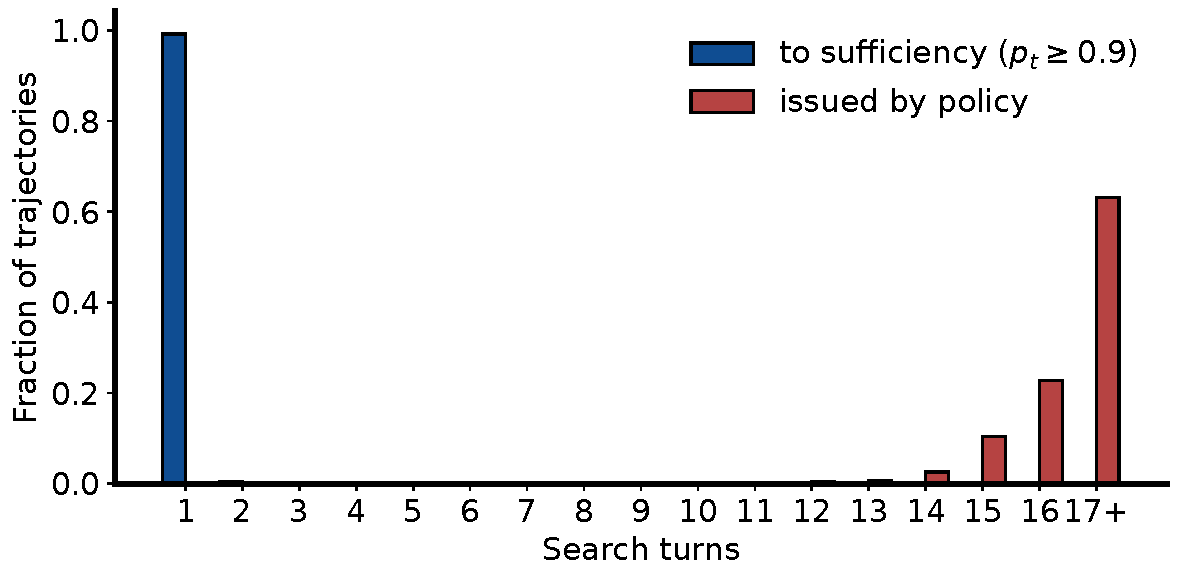
\includegraphics[width=0.72\textwidth]{fig_searches_vs_sufficiency.pdf}
\caption{Searches needed (first $p_t \geq 0.9$; blue) versus searches issued (red), fraction of
trajectories. Sufficiency is concentrated at one search on this single-hop slice; issued
searches concentrate at the horizon.}
\label{fig:suff}
\end{figure}

\subsection{The repeated-query attractor}\label{sec:attractor}
Criterion failures are sharply position-dependent (Fig.~\ref{fig:fail}, Table~\ref{tab:fail}).
The first search is nearly always sensible; by position $\geq 3$, \code{novel} fails on
99.96\% of turns and \code{info\_gain} on 99.98\%: the policy re-issues the same or a
near-duplicate query and re-retrieves the same documents. The mean longest consecutive
non-novel run is \textbf{16.0 turns}; 99.95\% of trajectories contain a run of $\geq 3$.
By contrast, \code{well\_formed} (92.6\%) and \code{relevant} (10.8\%) failure rates are flat
in position: they measure query \emph{style} (the policy pastes the question verbatim
everywhere) and topicality, not the loop. The attractor is fully captured by
\code{novel}/\code{info\_gain}/\code{progression}.

\begin{figure}[h]\centering
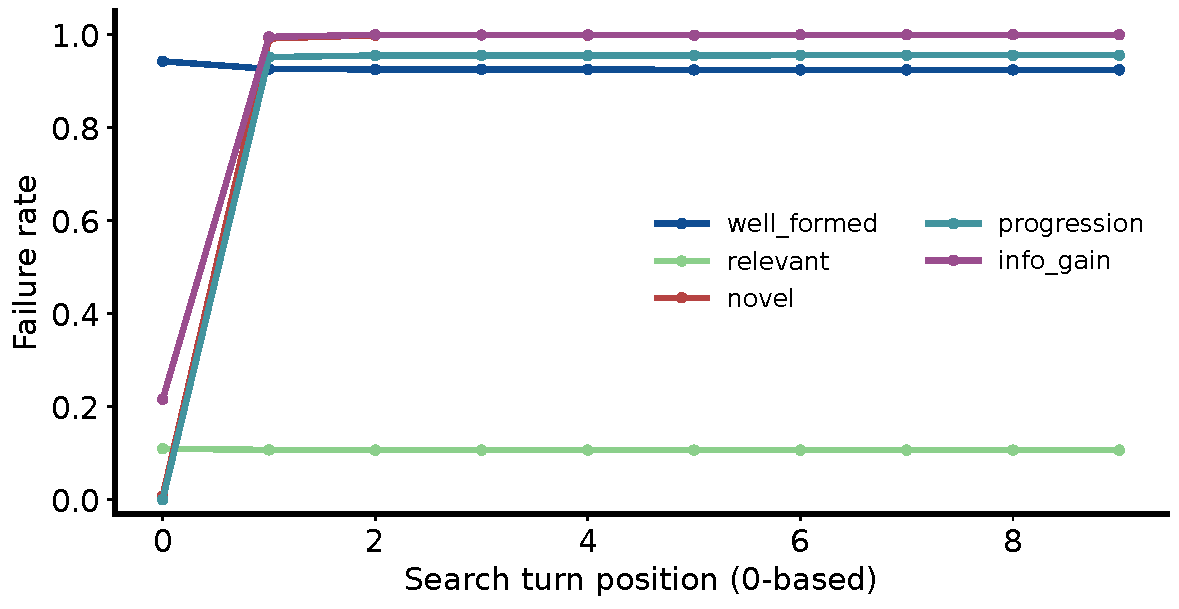
\includegraphics[width=0.66\textwidth]{fig_criterion_fail.pdf}
\caption{Criterion failure rate by search-turn position. The loop criteria
(\code{novel}, \code{info\_gain}, \code{progression}) jump from $\approx 0$ to $\approx 1$
after the first search; the style criteria (\code{well\_formed}, \code{relevant}) are
position-independent.}
\label{fig:fail}
\end{figure}

\begin{table}[h]\centering\small
\begin{tabular}{lrrr}
\toprule
\textbf{Criterion} & \textbf{fail@turn 0} & \textbf{fail@turns $\geq$3} & \textbf{fail, all turns}\\
\midrule
\code{novel}       & 0.008 & 0.9996 & 0.941\\
\code{info\_gain}  & 0.216 & 0.9998 & 0.954\\
\code{progression} & 0.000 & 0.956  & 0.900\\
\code{well\_formed}& 0.943 & 0.925  & 0.926\\
\code{relevant}    & 0.110 & 0.108  & 0.108\\
\bottomrule
\end{tabular}
\caption{Position dependence of criterion failures (34{,}125 turns).}
\label{tab:fail}
\end{table}

\subsection{Readiness dynamics}
Mean $p_t$ by position, split by outcome (Fig.~\ref{fig:ready}): successful trajectories
saturate readiness at the first search ($p \approx 0.9$ at position 0) and stay flat ---
subsequent searches add nothing the judge can see. Failed trajectories plateau near 0.5 and
never recover, consistent with ``retrieved the wrong entity's page and kept re-retrieving it''
rather than progressive refinement. $p_0 = 0$ for every trajectory.

\begin{figure}[h]\centering
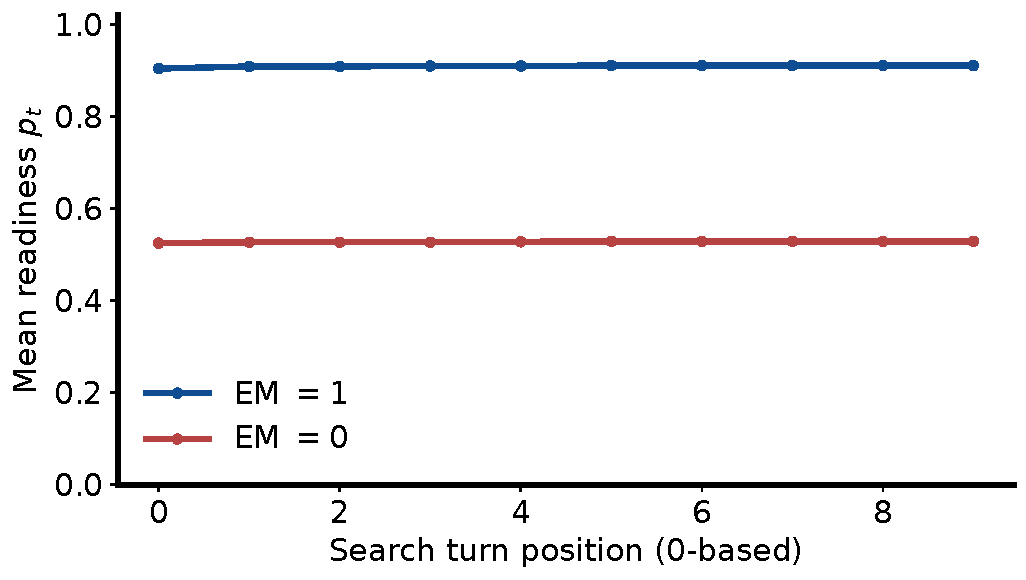
\includegraphics[width=0.6\textwidth]{fig_readiness.pdf}
\caption{Mean readiness $p_t$ by turn position and final outcome.}
\label{fig:ready}
\end{figure}

\subsection{Which judge signals predict success?}\label{sec:auc}
Rank AUC of trajectory-level signals against EM (Fig.~\ref{fig:auc}): $p_{final}$ 0.74 and mean
\code{info\_gain} 0.69 carry real signal; \code{novel}/\code{progression}/\code{relevant}
$\approx$0.56 are weakly informative individually on this single-hop slice; raw search count is
similarly weak (0.56, fewer-is-better). \code{well\_formed} is at chance (0.49): it fires
near-uniformly on wins and losses alike.

\begin{figure}[h]\centering
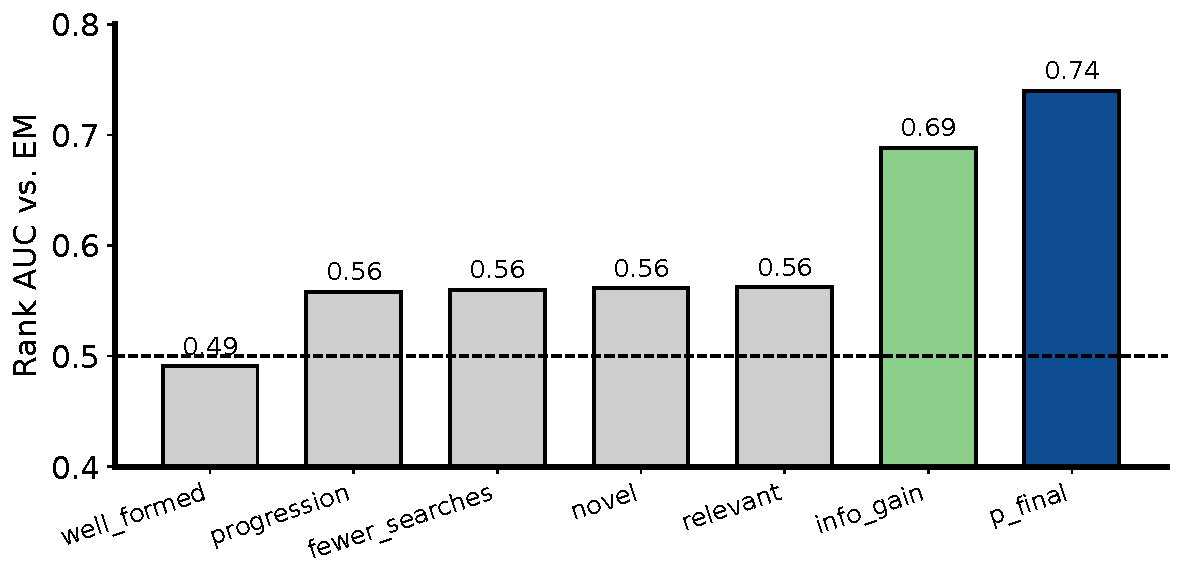
\includegraphics[width=0.66\textwidth]{fig_auc.pdf}
\caption{Predicting trajectory success (EM): rank AUC per judge signal. Dashed line = chance.}
\label{fig:auc}
\end{figure}

\section{Implications for the reward arms}
\begin{itemize}
\item \textbf{pen (asymmetric penalties).} The actionable penalty surface is
\code{novel}$=0$ (position-targeted, mechanism-aligned; \S\ref{sec:attractor}) and
$t > \code{sufficiency\_turn}$ (66\% of turns; \S\ref{sec:oversearch}).
\textbf{Drop \code{well\_formed} from the penalty}: at 92.6\% uniform failure and AUC 0.49 it
is a flat per-search tax --- behaviourally identical to the judge-free cost arm at vastly
higher compute --- and would dominate the summed penalty. Keep it as a logged canary.
\item \textbf{redist (return-equivalent redistribution).} $p_t$ saturates at the
evidence-finding turn, so increments $p_t - p_{t-1}$ concentrate credit exactly where intended
(the turn that found the evidence, not the spin). AUC 0.74 for $p_{final}$ supports the
signal; formal calibration (reliability of $p$ vs.\ empirical solve rate) runs on the
temperature-1.0 collection.
\item \textbf{cost (judge-free control).} The attractor gives even a blind per-search cost a
large target; the weak search-count AUC (0.56) is the a-priori case that \emph{which} searches
get cut matters --- i.e.\ why pen may retain accuracy better than cost.
\item \textbf{Judge operations.} JSON-schema mode: 0/2{,}000 fallbacks; $\sim$45 min for
2{,}000 trajectories on 4$\times$H100 at concurrency 32 --- comfortably inside the
$\sim$6M input-token/step budget for training-time judging (1{,}280 trajectories/step).
\end{itemize}

\section{Limitations}
\begin{itemize}
\item \textbf{Greedy decoding.} Repetition attractors are amplified at temperature 0; the
training-time profile is $\sim$5.4 searches/rollout at temperature 1.0. Magnitudes here are an
upper bound; the position-dependence \emph{shape} is the transferable finding. The
temperature-1.0 collection from baseline checkpoints 25/50/75 (in flight) is the
training-matched replication.
\item \textbf{Single-hop slice.} The 2{,}000-trajectory cap covers NQ + TriviaQA only;
\code{progression} is rarely exercised and sufficiency lands on the first search partly by task
construction. Multi-hop criterion behaviour (HotpotQA, 2Wiki, Musique) is unmeasured here.
\item \textbf{Judge as ground truth.} Criterion ``failure rates'' are judge assessments; the
Phase-1 launch gate includes a manual precision spot-check ($\sim$100 trajectories,
$\geq$80\% precision per criterion) before any flag earns a gradient.
\item \textbf{Sufficiency $\neq$ answerability.} $p_t \geq 0.9$ is the judge's evidence
estimate given gold answers; a policy cannot see $p_t$ and must learn stopping from the reward.
\end{itemize}

\section{Reproducibility}
Branch \code{judge-reward-arms} (repo \code{Agentic-RL-CA}), report directory
\code{docs/reports/2026-08-14\_rubric\_error\_patterns/}. Figures pair with their data as
\code{assets/fig\_*.pdf} + \code{assets/fig\_*.csv}.
\begin{itemize}
\item Rubric judging (4$\times$H100 worker, serves gpt-oss-120b + judges the dump):\\
\code{DUMPS="grpo\_s75=\$HLOG/p8b\_eval\_grpo\_s75/rollout\_eval\_grpo\_s75.jsonl.zst"}\\
\code{GOLDSET=.../asearcher\_eval.parquet MAX\_TRAJS=2000 bash scripts/asearcher/p8b\_rubric\_judge\_worker.sh}
\item This paper's statistics and figures: \code{uv run make\_paper\_figs.py}; the HTML
companion report: \code{index.html} (same directory).
\end{itemize}

\end{document}
